\item ¿Cuál es la ip de la Interfaz que ha recibido el mayor número de octetos?

Primero listamos en la figura \ref{image:octetos} los octetos que han recibido cada una de las interfaces. Esto nos devuelve en índice del objeto correspondiente a cada interfaz.

\FloatBarrier
\begin{figure}[htbp!]
		\centering
			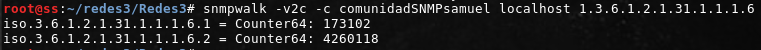
\includegraphics[width=.9 \textwidth]{images/7-linux-1}
		\caption{Octetos por interfaz.}
		\label{image:octetos}
\end{figure}
\FloatBarrier

Observamos que la interfaz que ha recibido más octetos es la que tiene el índice 2. Por lo tanto, procedemos listar las interfaces por índice mostrando su dirección IP, tal y como se muestra en la figura \ref{image:ips}.

\FloatBarrier
\begin{figure}[htbp!]
		\centering
			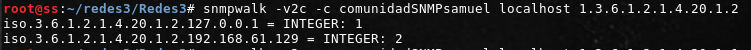
\includegraphics[width=.9 \textwidth]{images/7-linux-2}
		\caption{Direcciones IP de cada interfaz.}
		\label{image:ips}
\end{figure}
\FloatBarrier

Obtenemos que, la dirección IP de la interfaz que ha recibido más octetos es la dirección 192.168.61.129.

Repetimos el procedimiento anterior para el caso de Windows. Con respecto al número de octetos recibidos por cada interfaz obtenemos lo mostrado en la figura \ref{image:octetos-windows}, mientras que la lista de direcciones IP se muestra en la figura \ref{image:ips-windows}.

\FloatBarrier
\begin{figure}[htbp!]
		\centering
			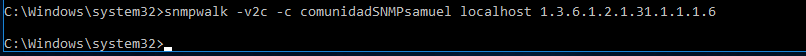
\includegraphics[width=.9 \textwidth]{images/7-windows-1}
		\caption{Octetos por interfaz.}
		\label{image:octetos-windows}
\end{figure}
\FloatBarrier

\FloatBarrier
\begin{figure}[htbp!]
		\centering
			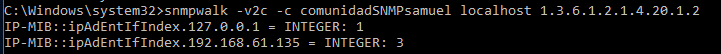
\includegraphics[width=.9 \textwidth]{images/7-windows-2}
		\caption{Direcciones IP de cada interfaz.}
		\label{image:ips-windows}
\end{figure}
\FloatBarrier

Sin embargo, obtenemos que, el número de octetos recibidos por cada interfaz no está definido.

\item ¿Cuántos mensajes ICMP ha recibido el agente?

En la figura \ref{image:icmp-linux} observamos que el número de mensajes que ha recibido el agente Linux es de 1. Mientras que, en la figura \ref{image:icmp-windows} observamos que el número de mensajes que ha recibido el agente Windows es de 0.

\FloatBarrier
\begin{figure}[htbp!]
		\centering
			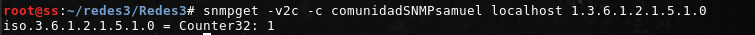
\includegraphics[width=.9 \textwidth]{images/8-linux}
		\caption{Mensajes ICMP recibidos en Linux.}
		\label{image:icmp-linux}
\end{figure}
\FloatBarrier

\FloatBarrier
\begin{figure}[htbp!]
		\centering
			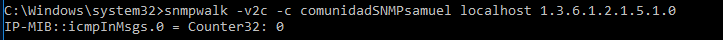
\includegraphics[width=.9 \textwidth]{images/8-windows}
		\caption{Mensajes ICMP recibidos en Windows.}
		\label{image:icmp-windows}
\end{figure}
\FloatBarrier

\item ¿Cuántas entradas tiene la tabla de enrutamiento IP?

Para responder esta pregunta, basta con listar y contar el número de entradas en alguna de las columnas de la tabla ipRouteTable. En este caso, utilizamos el objeto ipRouteDest.

En la figura \ref{image:route-linux} observamos que el número de entradas de ipRouteTable del agente Linux es de 2. Mientras que, en la figura \ref{image:route-windows} observamos que el número de entradas de ipRouteTable del agente Windows es de 9.

\FloatBarrier
\begin{figure}[htbp!]
		\centering
			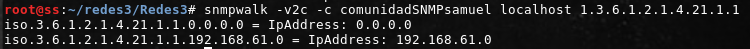
\includegraphics[width=.9 \textwidth]{images/9-linux}
		\caption{Entradas en ipRouteTable en Linux.}
		\label{image:route-linux}
\end{figure}
\FloatBarrier

\FloatBarrier
\begin{figure}[htbp!]
		\centering
			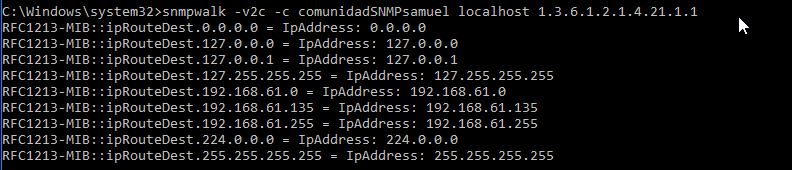
\includegraphics[width=.9 \textwidth]{images/9-windows}
		\caption{Entradas en ipRouteTable en Windows.}
		\label{image:route-windows}
\end{figure}
\FloatBarrier